\documentclass[tikz,border=7pt]{standalone}
\usepackage[T1]{fontenc}
\usepackage{lmodern}
\usepackage{helvet}
\renewcommand{\familydefault}{\sfdefault}
\usepackage[table]{xcolor}
\usepackage{tikz}
\usetikzlibrary{arrows.meta,positioning,calc}
\definecolor{ink}{HTML}{163B60}
\definecolor{wash}{HTML}{E4F1FC}
\tikzset{box/.style={draw=ink,rounded corners=3pt,line width=.8pt,minimum height=1cm,align=center,inner sep=8pt},flow/.style={-{Stealth[length=2.5mm]},draw=ink,line width=1pt},font=\sffamily\normalsize,every node/.style={text=ink}}
\begin{document}
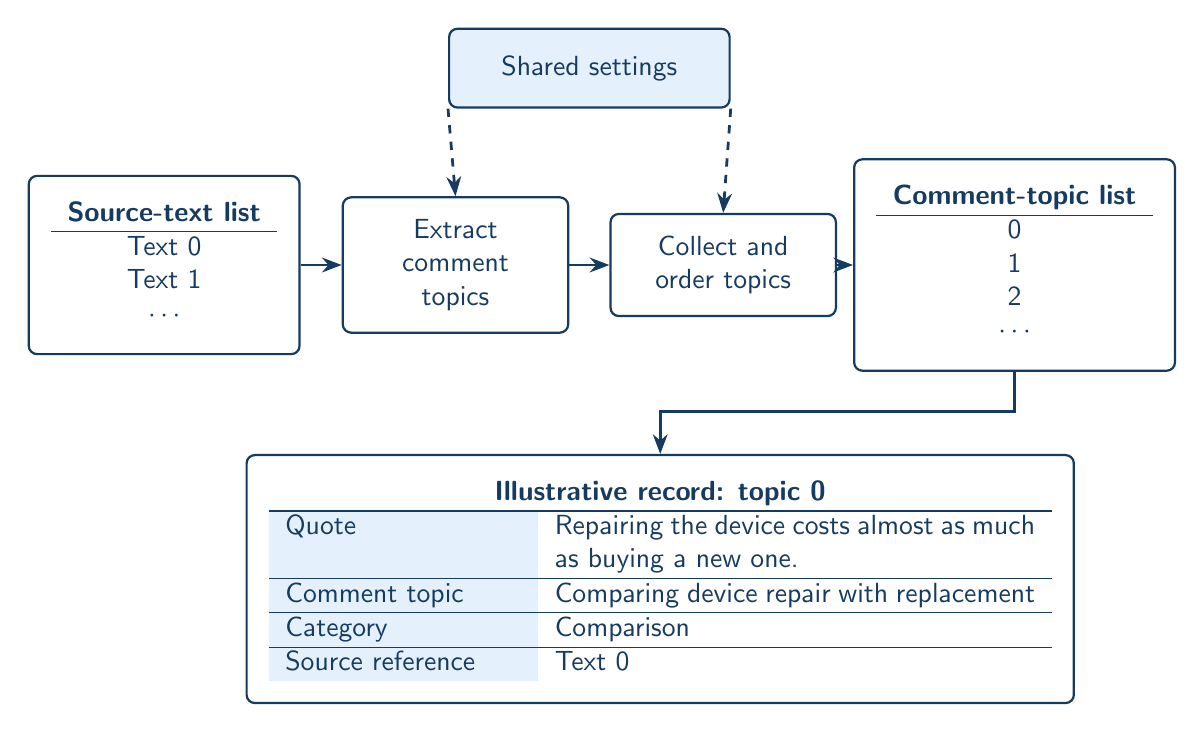
\begin{tikzpicture}
\node[box] (texts) at (0,0) {\begin{tabular}{c}\textbf{Source-text list}\\\hline Text 0\\Text 1\\$\cdots$\end{tabular}};
\node[box,text width=2.3cm] (extract) at (3.7,0) {Extract\\comment topics};
\node[box,text width=2.3cm] (order) at (7.1,0) {Collect and\\order topics};
\node[box] (topics) at (10.8,0) {\begin{tabular}{c}\textbf{Comment-topic list}\\\hline 0\\1\\2\\$\cdots$\end{tabular}};
\node[box,fill=wash,text width=3cm] (setup) at (5.4,2.5) {Shared settings};
\draw[flow] (texts) -- (extract);
\draw[flow] (extract) -- (order);
\draw[flow] (order) -- (topics);
\draw[flow,dashed] (setup.south west) -- (extract.north);
\draw[flow,dashed] (setup.south east) -- (order.north);
\node[box,anchor=north] (example) at (6.3,-2.4) {\begin{tabular}{p{3cm}p{6.1cm}}\multicolumn{2}{c}{\textbf{Illustrative record: topic 0}}\\\hline
\cellcolor{wash}Quote & Repairing the device costs almost as much as buying a new one.\\\hline
\cellcolor{wash}Comment topic & Comparing device repair with replacement\\\hline
\cellcolor{wash}Category & Comparison\\\hline
\cellcolor{wash}Source reference & Text 0\\
\end{tabular}};
\draw[flow] (topics.south) -- ++(0,-.5) -| (example.north);
\end{tikzpicture}
\end{document}
